% -*- TeX:SI -*-
% slovene sub-mode for spell check
%%%%%%%%%%%%%%%%%%%%%%%%%%%%%%%%%%%%%%%%%%%%%%%%%%%%%%%%%%%%%%%%%%%%%%%%%%%%%%%%%%%%%%%%%%%%%%%%%%%%%%%%%%%%%%%%%%%%%%%%
% LaTeX predloga za zaključna dela
% Univerza v Ljubljani, Fakulteta za elektrotehniko
% Zbral in uredil: Roman Kamnik, junij 2013
% Dopolnil: Sebastjan Šlajpah (2013), Sašo Tomažič (2013), Peter Miklavčič (2019)
%%%%%%%%%%%%%%%%%%%%%%%%%%%%%%%%%%%%%%%%%%%%%%%%%%%%%%%%%%%%%%%%%%%%%%%%%%%%%%%%%%%%%%%%%%%%%%%%%%%%%%%%%%%%%%%%%%%%%%%%
\documentclass[a4paper,twoside,openright,12pt,slovene]{book}
\usepackage[pdftex]{UNI-LJ-FE-Diploma} % stil zaključnega dela UL FE
\usepackage[utf8]{inputenc} % predloga uporablja standardno kodiranje Unicode UTF-8, ki podpira šumnike
\usepackage[greek,english,slovene]{babel} % seznam uporabljenih jezikov (zadnji na seznamu je primarni)
\usepackage[utf8]{inputenc}
\usepackage{subcaption}

% Default fixed font does not support bold face
\DeclareFixedFont{\ttb}{T1}{txtt}{bx}{n}{12} % for bold
\DeclareFixedFont{\ttm}{T1}{txtt}{m}{n}{12}  % for normal

\usepackage{minted}
% PDF/A %%%%%%%%%%%%%%%%%%%%%%%%%%%%%%%%%%%%%%%%%%%%%%%%%%%%%%%%%%%%%%%%%%%%%%%%%%%%%%%%%%%%%%%%%%%%%%%%%%%%%%%%%%%%%%%%
% Več o PDF/A v LaTeX-u: https://www.mathstat.dal.ca/~selinger/pdfa/
\usepackage{filecontents}
\begin{filecontents*}{\jobname.xmpdata}
    \Title{Uporaba strojnega vida za izboljšanje kolaborativne robotike} % Mora biti enak kot je v prijavi teme!
    \Author{Gašper Šavle} % Mora biti enak kot na naslovnici!
\end{filecontents*}
\usepackage[a-1b]{pdfx}
%%%%%%%%%%%%%%%%%%%%%%%%%%%%%%%%%%%%%%%%%%%%%%%%%%%%%%%%%%%%%%%%%%%%%%%%%%%%%%%%%%%%%%%%%%%%%%%%%%%%%%%%%%%%%%%%%%%%%%%%

% LaTeX PAKETI %%%%%%%%%%%%%%%%%%%%%%%%%%%%%%%%%%%%%%%%%%%%%%%%%%%%%%%%%%%%%%%%%%%%%%%%%%%%%%%%%%%%%%%%%%%%%%%%%%%%%%%%%
% Kompakten pregled LaTeX ukazov je dostopen na https://en.wikibooks.org/wiki/Category:Book:LaTeX
% Navodila posameznih uporabljenih paketov so dostopna na https://www.ctan.org

% Dodatni simboli
\usepackage{textcomp}                               % dodatni simboli (kot npr. €)
\usepackage{gensymb}                                % dodatni simboli \de­gree, \cel­sius, \pert­hou­sand, \mi­cro, \ohm
\newcommand{\uppi}{\textrm{\greektext p\latintext}} % velika grška črka P z \uppi, alternativa simbolu \Pi

% Osnovno oblikovanje
% dodatne možnosti hiperpovezav
\usepackage[normalem]{ulem}                          % podčrtavanje in prečrtavanje teksta
\usepackage{float}                                   % dodatne možnosti oblikovanja objektov
\usepackage{enumitem}                                % dodatne možnosti oblikovanja seznamov

% Dodatno oblikovanje
%\zamaknirobsodihstrani{0mm} % dodatna prilagoditev levega roba sodih strani za dvostranski tisk
%\usepackage{dcolumn}        % poravnava po decimalnih mestih v tabelah
%\usepackage{longtable}      % večstranske tabele
%\usepackage{caption}        % dodatne možnosti označevanja objektov
%\usepackage{rotating}       % vretenje objektov, strani, ipd.

% Matematična orodja
\usepackage{mathtools} % http://mirrors.ctan.org/macros/LaTeX/contrib/mathtools/mathtools.pdf
\usepackage{bm}        % ukaz za odebeljeni tisk \bm v matematičnih okoljih
%\usepackage{cancel}   % ukaz za prečrtavanje \cancel v matematičnih okoljih

% Grafična orodja
\usepackage{graphicx}                 % vključevanje bitnih slik z ukazom \includegraphics
\usepackage{grffile}                  % podpora presledkom pri ukazu \includegraphics
%\usepackage{tikz}                    % paket TikZ za risanje (npr. blokovnih shem, diagramov poteka, itd.)
%\usetikzlibrary{calc,shapes,arrows}  % dodatne možnosti paketa TikZ
%\usepackage{tikzscale}               % skaliranje risb
%\usepackage[smartlabels]{circuitikz} % risanje shem vezij
%\usepackage{pgfplots}                % paket PGFPlots za risanje grafov, tudi iz CSV in podobnih datotek
%\usepgfplotslibrary{polar,external}  % dodatne možnosti paketa PGFPlots
%\usepackage{tikz-3dplot}             % 3D risanje
% Primeri: http://texample.net , http://pgfplots.net/tikz/examples , http://pgfplots.sourceforge.net/gallery.html

% Vključevanje datotek
\usepackage{pdfpages} % vključevanje PDF datotek z ukazom \includegraphics
\usepackage{epstopdf} % vključevanje EPS datotek z ukazom \includegraphics
\usepackage{listings} % orodja za izpisovanje programske kode
\lstset{              % nastavitve orodja za izpisovanje programske kode
    basicstyle=\ttfamily\footnotesize,
    breaklines=true,
    numbers=left,
    numberstyle=\scriptsize,
    keywordstyle=\color{blue},
    commentstyle=\color{unilj},
    stringstyle=\color{olive},
}
%%%%%%%%%%%%%%%%%%%%%%%%%%%%%%%%%%%%%%%%%%%%%%%%%%%%%%%%%%%%%%%%%%%%%%%%%%%%%%%%%%%%%%%%%%%%%%%%%%%%%%%%%%%%%%%%%%%%%%%%

% DEKLARACIJE %%%%%%%%%%%%%%%%%%%%%%%%%%%%%%%%%%%%%%%%%%%%%%%%%%%%%%%%%%%%%%%%%%%%%%%%%%%%%%%%%%%%%%%%%%%%%%%%%%%%%%%%%%
\naslov{Uporaba strojnega vida za izboljšanje kolaborativne robotike} % Mora biti enak kot je v prijavi teme!
\avtor{Gašper Šavle} % Mora se ujemati s \Title pri metapodatkih PDF/A!
\mentor{Prof.Dr. Aleš Ude}
%\somentor{Naziv, ime in priimek somentorja}
\date{Ljubljana, \the\year}
\univerza{Univerza v Ljubljani}
\definecolor{unilj}{cmyk}{0.00, 0.94, 0.94, 0.06} % barva Univerze v Ljubljani

% Potrebno je paziti, da je izbrana prava kombinacija tipa dela in sodelujočih fakultet glede na študijski program!
%\delo{Diplomsko delo\\~\\Univerzitetni študijski program prve stopnje Elektrotehnika}
%\delo{Diplomsko delo\\~\\Univerzitetni študijski program prve stopnje Multimedija}
\delo{Diplomsko delo\\~\\Visokošolski strokovni študijski program\\prve stopnje Aplikativna elektrotehnika}
%\delo{Diplomsko delo\\~\\Visokošolski strokovni študijski program\\prve stopnje Multimedijske komunikacije}
%\delo{Magistrsko delo\\~\\Magistrski študijski program druge stopnje Elektrotehnika}
%\delo{Magistrsko delo\\~\\Magistrski študijski program druge stopnje Uporabna statistika}
\fakulteta{Fakulteta za elektrotehniko}
%\fakulteta{Fakulteta za elektrotehniko,\\Fakulteta za računalništvo in informatiko} % Za program Multimedija
%\fakulteta{Fakulteta za elektrotehniko, Biotehniška fakulteta,\\Ekonomska fakulteta, Fakulteta za družbene vede,\\Fakulteta za matematiko in fiziko, Fakulteta za\\računalništvo in informatiko, Medicinska fakulteta} % Za program Uporabna statistika
%%%%%%%%%%%%%%%%%%%%%%%%%%%%%%%%%%%%%%%%%%%%%%%%%%%%%%%%%%%%%%%%%%%%%%%%%%%%%%%%%%%%%%%%%%%%%%%%%%%%%%%%%%%%%%%%%%%%%%%%

% DOKUMENT %%%%%%%%%%%%%%%%%%%%%%%%%%%%%%%%%%%%%%%%%%%%%%%%%%%%%%%%%%%%%%%%%%%%%%%%%%%%%%%%%%%%%%%%%%%%%%%%%%%%%%%%%%%
\begin{document}
\frontmatter

\selectlanguage{slovene}

%******************************* NASLOVNICA ************************************
\maketitle

%******************************* ZAHVALA ***************************************
\zahvala
V zahvali se kandidat lahko zahvali mentorju in poimensko tudi vsem sodelavcem in prijateljem, ki so pomagali in prispevali pri delu v laboratoriju, na računalniku, v delavnici, pri tehnični izdelavi dela ali drugje.
(najverjetneje je na koncu ne bom mel ampak bomo videli kolikomateriala uspem nabrat)

%******************************* POVZETEK IN KLJUČNE BESEDE ********************
\povzetek
Kolaborativna robotika je vedno hitreje rastoca podzvrst industrijske robotike, do leta 2027 anj bi trg kolaborativne robotike dosegel vrednost 7,5 milijarde ameriskih dolarjev, predstavljal pa naj bi kar 29\%
trga industrijske robotike.
To eksplozivno rast poganjajo stevilni aktualni dejavniki, kot so pomanjkanje visoko usposobljenih delavcev, vedno vecja potreba po prilagodljivosti v avtomatiki in vedno manjse ter bolj raznolike serije izdelkov, ki se izdelujejo v industriji.

Sodelujoci roboti se od standardnih industrijskih robotov razlikujejo po zgradbi, saj so naceloma sestavljeni iz zaobljenih, ponekod celo mehkih clenov, ki so ob stiku s clovekom manj nevarni, kot njihove toge in oglate alternative. Druga najvecja razlika je vkljucitev senzorjev navora v sklepe robota, iz podatkov, ki jih robotski krmilnik razbere iz teh senzorjev je moc izracunati silo na posamezen sklep robota. Ti senzorji sile predstavljajo varnostno funkcijo zaznavanja trcenja med robotom in uporabnikom, ali robotom in zunanjimi objekti.

V diplomskem delu bom predstavil svojo izpeljavo uporabe strojnega vida za preprecevanje trcenj med clovekom in robotom, za kar sem uporabljal Intel Realsense stereoskopsko kamero in Franka Emika Panda robota. Uporabil sem program za zaznavanje drze in polozaja cloveka AlphaPose, s katerim sem pridobil podatke o polozaju posameznega sklepa cloveka v koordinatnem sistemu kamere. Podatke sem nato s transformacijsko matriko preslikal v izvorni koordinatni sistem "world", v katerem je definiran tudi polozaj robotov. Ko robotski kmilnik zazna vnaprej doloceno razdaljo med robotom in clovekom, za katero je bilo razsojeno, da signalizira nevernost trcenja, upocasni gibanje robota na hitrost, ob kateri trk s clovekom ne bi bil nevaren.

\textbf{TODO:} 
- opis trenutnih resitev (glej bookmarks/diplomska) in citati iz teh clankov, oceni pomembnost za diplomsko
- rezultati in zakljucki iz rezultatov

\kljucnebesede
Sodelujoci roboti, zaznavanje drze, robotski krmilnik, AlphaPose, transformacijska matrika, koordinatni sistem

\tableofcontents

%******************************* SEZNAM SLIK, SEZNAM TABEL *********************
\seznamslik
\seznamtabel

%******************************* SEZNAM SIMBOLOV *******************************
\seznamsimbolov
V pričujočem zaključnem delu so uporabljene naslednje veličine in simboli:

\begin{center}
    \begin{tabular}{*{4}{l}} \hline
        \multicolumn{2}{c}{\bf{Veličina / oznaka}}           & \multicolumn{2}{c}{\bf{Enota}} \\ \hline
        Ime                & Simbol                          & Ime      & Simbol              \\ \hline
        čas                & $t$                             & sekunda  & s                   \\
        frekvenca          & $f$                             & Hertz    & Hz                  \\
        tlak               & $p$                             & Pascal   & Pa                  \\
        sila vzgona        & $\textbf{\textit{F}}_\text{vz}$ & Newton   & N                   \\
        gostota            & $\rho$                          & -        & kg/m$^3$            \\
        masa               & $m$                             & kilogram & kg                  \\
        vhodna napestost   & $U_\text{vh}$                   & volt     & V                   \\
        Jacobijeva matrika & $\mathbf{J}$                    & -        & -                   \\ \hline
    \end{tabular}
\end{center}

Pri čimer so vektorji in matrike zapisani s poudarjeno pisavo. Natančnejši pomen simbolov ter njihovih indeksov je razviden iz ustreznih slik ali pa je pojasnjen v spremljajočem besedilu, kjer je simbol uporabljen.

\mainmatter

%******************************* UVOD ******************************************
\chapter{Uvod} \label{uvod}

Uvod v zaključno delo ima namen, da uvede bralca v tematiko zaključnega dela. V njem kandidat razčleni zahteve in cilje zaključnega dela, po literaturi povzame znane rešitve in oceni njihov pomen za zaključno delo. Sklicevanje na literaturo se v besedilu označi s številko v oglatem oklepaju, ki jo ima ta v seznamu uporabljenih virov, in po potrebi navede strani, npr. \cite{miklavcic2010objavljanje} ali \cite[stran 520-534]{juznic1992diplomska}.

Obstojece resitve:
V industriji se za zaznavanja cloveka v delovnem prostoru robota (ali katerekoli naprave) najpogosteje uporablja svetlobne zavese \ref{svetlobna_zavesa} ali ultrazvocne senzorje prisotnosti/razdalje. Tezava obojih pristopov je kompleksnost prvotne nastavitve takega sistema in njegova fleksibilnost. Npr. da svetlobna zavesa pravilno deluje morajo biti vsi sprejemniki in oddajniki popolnoma poravnani, dobimo pa le binarni izhod, ki nam pove, ali se nekaj trenutno nahaja znotraj ravnine, ki jo svetlobna zavesa tvori med svojima polovicama. To nam da zelo omejeno informacijo o trenutni lokaciji cloveka, kar nam tudi zelo omeji mozne odzive. Praviloma se ob motnji v svetlobni zavesi ustavi postroj, nakar sistem potrebuje uporabnisko interakcijo za ponovni zacetek normalnega delovanja postroja. Uporaba ultrazvocnih senzorjev oddaljenosti, lahko dobimo vecstopenjsko informacijo o blizini dolocenega objekta, vendar moramo tocno vedeti, kje bi se ta objekt (v tem primeru clovek) lahko nahajal. Sistem se ne zaveda, kaj je objekt, cigar razdaljo merimo, kar nam lahko predstavi motnje v meritvah, ki pa vodijo do nezanesljivega delovanje.

\begin{figure}[h]
    \centering
    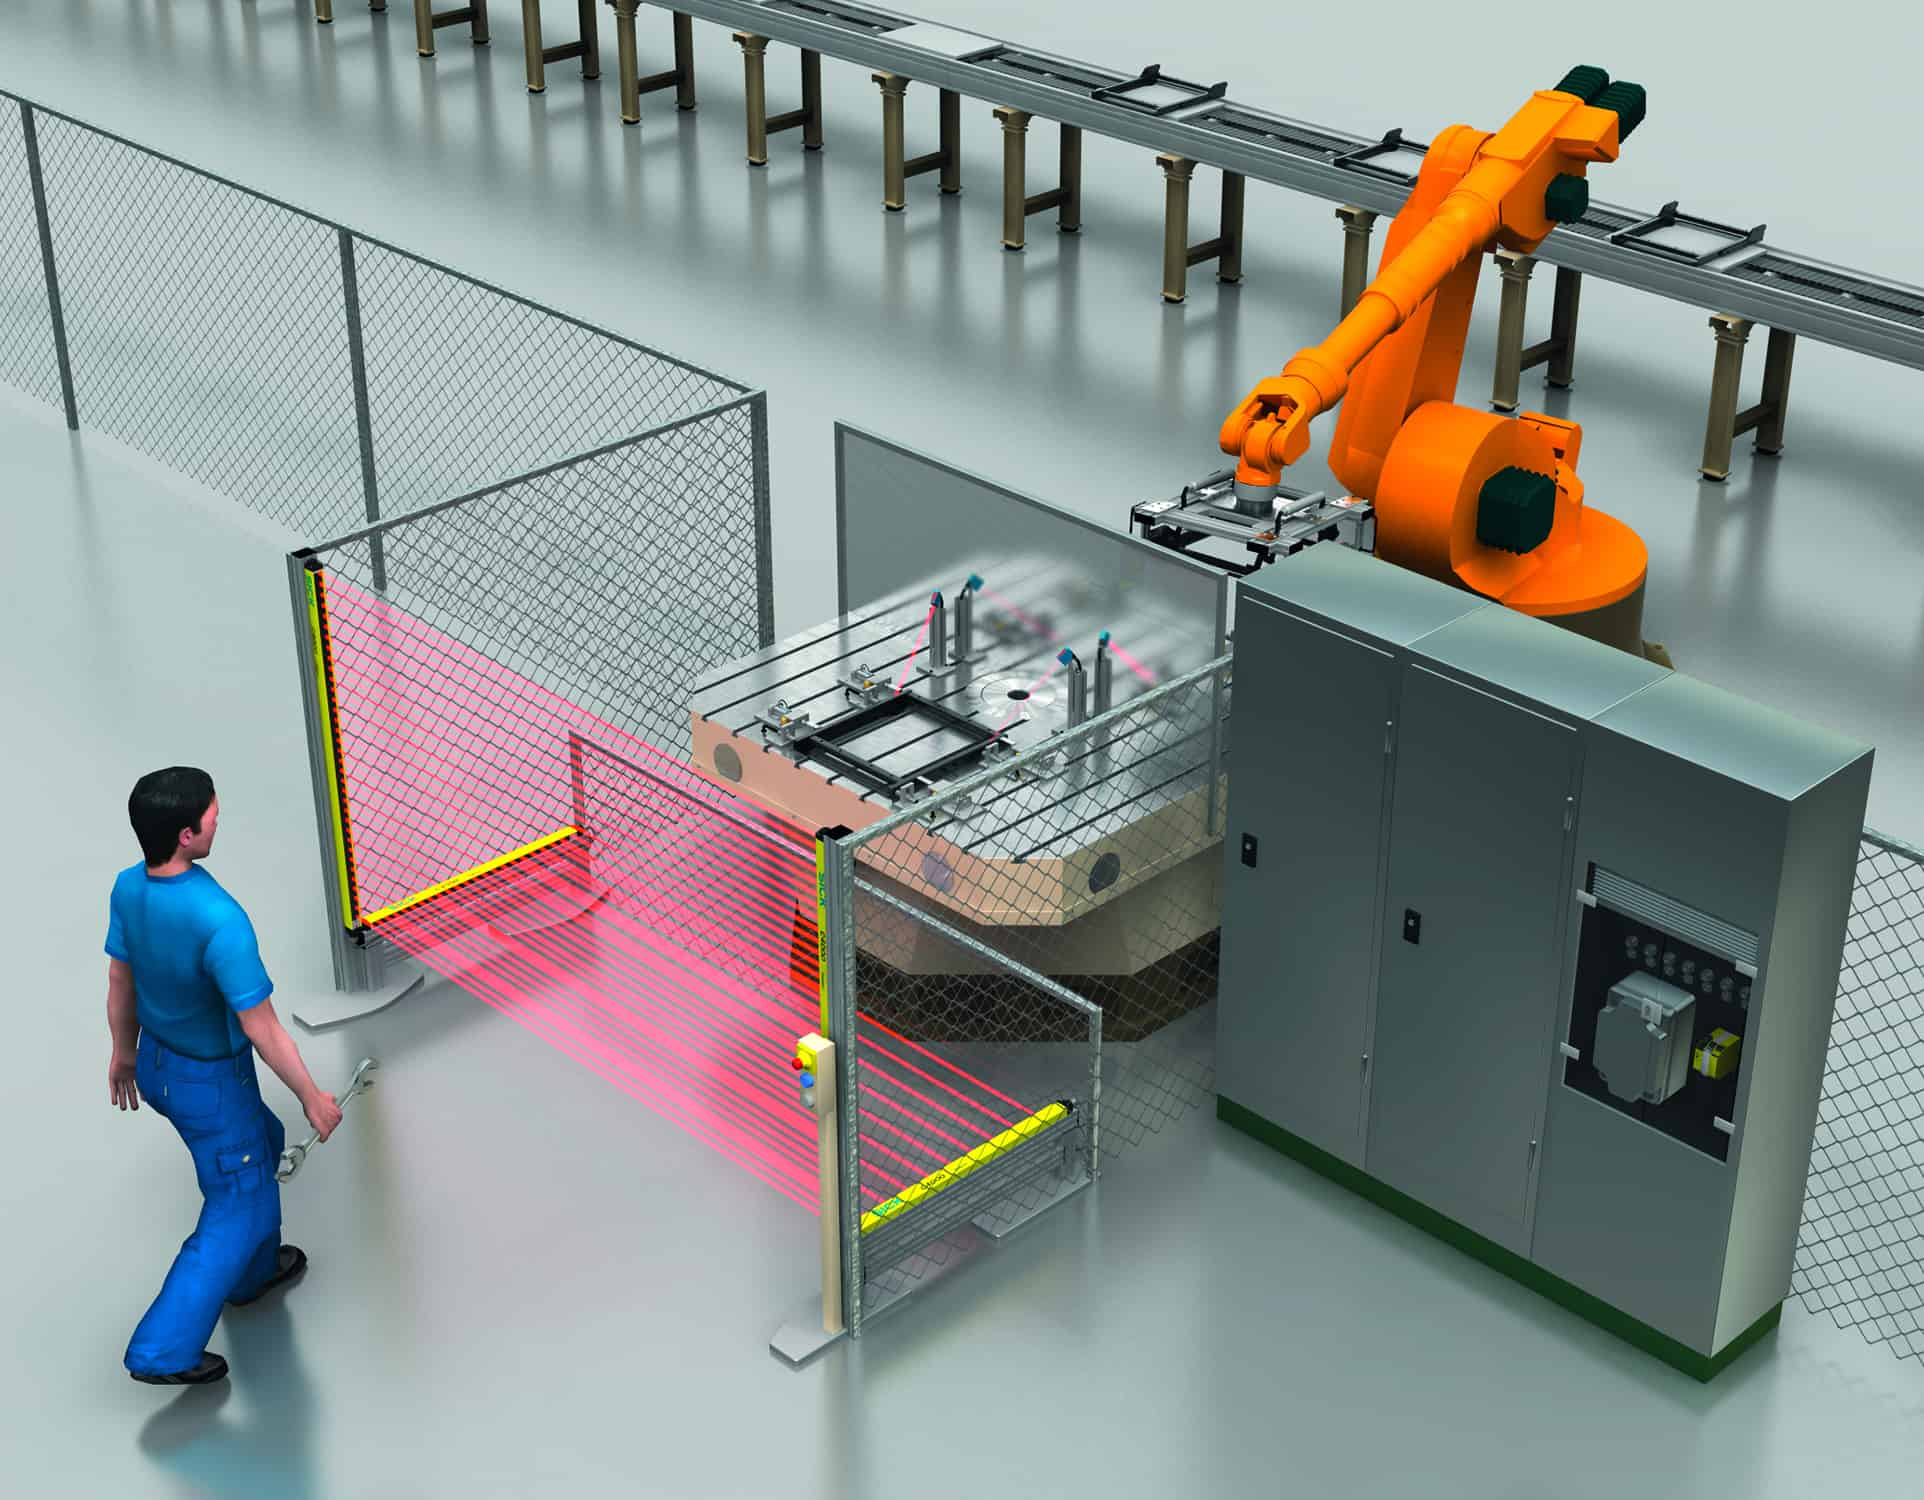
\includegraphics[width=0.75\columnwidth]{Slike/light-curtain-application.jpg}
    \caption{\label{svetlobna_zavesa} Primer svetlobne zavese v industriji.}
\end{figure}

Prednost uporabe strojnega vida napram tradicionalnim resitvam, kot so svetlobne zavese ali ultrazvocni merilniki razdalje je informacija o tem, kaj tocno se nahaja v delavnem prostoru in nasplosno vecji nabor podatkov, na bazi katerih lahko sprogramiramo kompleksnejse odzive.

\chapter{Predstavitev sestavnih delov resitve} \label{opis_komponent}
\section{Robotski operacijski sistem (ROS)} \label{ROS}
ROS (Robot Operating System) je odprtokodni operacijski sistem, zasnovan za uporabo v robotskih aplikacijah. Deluje na računalnikih z operacijskim sistemom Linux in je zasnovan na distribucijski arhitekturi. Torej, da je zasnovan za delovanje na različnih računalnikih, ki lahko delujejo, kot povezana celota - sistem. Ker je moja tema diplomske naloge nadgradnja obstojecega projekta na IJS, kjer sem opravljal obvezno prakso, sem moral resitev narediti kompatibilno z njihovo obstoječo arhitekturo projekta, kjer se vse nahaja v Docker datotekah, oz. Dockerfile-ih. Torej sem tudijaz svojo resitev zgradil znotraj Docker containerja, kar je tudi sicer priporocljivo v praksi, zaradi lazjega upravljanja s knjiznicami in gonilniki. 

\textbf{TODO: Narisi shemo delovanja ROS}

Arhitekturo ROS \cite{ROS_arhitektura} lahko razumemo na dveh razlicnih nivojih, ki ju lahko poenostavimo v:
\begin{enumerate}
    \item  \label{file_lvl} \textbf{Datotecni (Filesystem) nivo} 
    
    Nivo datotečnega sistema je najnizji nivo operacijskega sistema, opisuje njegovo interno strukturo in je namenjen centralizaciji gradnikov projekta, vendar obenem zadostni fleksibilnosti, da je moč decentralizirati potrebe vsakega gradnika. ROS operacijski sistem je razdeljen v mape, ki vsebujejo datoteke, v katerih je opisana njihova funkcija. Funkcije datotek pa ločimo na:
        \begin{itemize}
            \item \textbf{Pakete (packages):} Najnižje-nivojska komponenta ROS, vsebuje minimalno strukturo, ki je potrebna za stvarjenje programa znotraj operacijskega sistema. Te strukture so lahko procesi ali konfiguracijske datoteke. Vsak paket potrebuje svoj \textit{manifest}, ki vsebuje informacije o paketu, kot npr. licence ali knjiznice, potrebne za delovanje.

            \item \textbf{Metapakete (metapackages):} Povezovalne strukture paketov, ki jih uporabljamo, ko hocemo vec paketov zbrati v vzajemno delujoco strukturo. Ta mapa vsebuje le datoteko \verb|package.xml|, ki vsebuje reference na pakete, ki jih zelimo skupinsko klicati. Metapaketi, kot osnovni paketi, prav tako potrebujejo svoj \textit{manifest}.

            \item \label{ros_msg} \textbf{Sporocila (messages):} Predstavljajo informacije, ki jih procesi posiljajo in prejemajo med sabo, ROS vsebuje vec standardnih tipov sporocil, mozna pa je nadgradnja z namenskimi tipi, ki jih lahko definiramo sami.

            \item \textbf{Storitve (services):} So nadgradnja sporocil [Glej: \ref{ros_msg}] in omogocajo poziv/odgovor (request/response) nacin komunikacije med vozlisci.[Glej: \ref{ros_node}] V sporocilu na katerem je zgrajena storitev so opisani vhodni in izhodni parametri storitve. Namenjene so izvajanju specificnih nalog ob klicu/na zahtevo
        \end{itemize}

 \item \label{block_lvl} \textbf{Blokovni nivo} 
 
 Nivo blokovne sheme ROS je nacin abstrakcije arhitekture ROS v visjenivojsko, uporabniku prijaznejso arhitekturo. Ta nivo je sestavljen iz skupka vseh procesov, kjer je vsak predstavljen, kot vozlisce, vsako vozlisce v tem omrezju procesov lahko dostopa do celotnega omrezja in komunicira s katerimkoli posameznim vozliscem. Na tem nivoju lahko procese locimo na:
    \begin{itemize}
        \item \label{ros_node}\textbf{Vozlišča (nodes):} Predstavljajo procese, kjer se obdelujejo podatki. Vsako vozlišče ima unikatno ime oziroma identifikator, ki ga določi programer ob inicializaciji vozlišča. Ta identifikator se uporablja za naslavljanje vozlišč ob komunikaciji med njimi. Vozlišča lahko komunicirajo prek tem ali storitev. Procese izvajamo v ločenih vozliščih za čim manjšo možnost kontaminacije, ko pride do napak ali neučinkovitosti v delovanju sistema. Tako kar se da preprečimo, da bi napaka v enem vozlišču okrnila delovanje ostalih.

        \item \label{ros_topic} \textbf{Teme (topics):} So asinhrona vodila, prek katerih vozlisca prenasajo podatke med sabo. So 'javna' domena, torej lahko prek njih komuncirajo vozlisca, ki niso neposredno povezana med sabo, kar pomeni, da sta posiljanje in branje podatkov lahko xasovno neodvisna. Tema ima lahko mnogo odjemalcev (subscribers) in mnogo ponudnikov (publishers), vendar lahko vecje stevilo ponudnikov na enem vodilu vodi do konfliktov. Ta sporocila se lahko posiljajo po TCP/IP ali UDP protokolu, izbiramo ju glede na potrebe aplikacije.

        \item \label{ros_service} \textbf{Storitve (services):} Tako kot teme, so tudi storitve mehanizem za komunikacijo med vozlisci. Vendar se mehanizma razlikujeta glede na namen in izvedbo. ROS service je namrec sinhron mehanizem za komunikacijo, kjer vozlisce zahteva informacijo od tocno dolocenega vozlisca in po poslanem pozivo (request) caka na odgovor, ki ga v obliki sporocila prejmemo, ko je klicana storitev opravljena.

        \item \label{ros_master} \textbf{Master:} Je odgovoren za imenovanje in ustvarjanje storitev in vseh ostalih vozlisc znotraj ROS operacijskega sistema. Usmerja pretok informacij med ponudniki in odjemalci. Njegova glavna vloga je omogocanje vozliscem, da se lahko med sabo najdejo in omogoca peer to peer [Glej: Razlaga pojmov - \ref{p_2_p}]. Prav tako pa upravlja s streznikom parametrov (parameter server) [Glej: \ref{ros_param}]

        \item \label{ros_param} \textbf{Streznik parametrov (parameter server):} Je slovar, dostopen celotnemu ROS sistemu, vozlisca ga uporabljajo za hranjenje, deljenje in dostop do parametrov med delovanjem. Vsak parameter je shranjen pod svojim unikatnim imenom. ROS sistemu omogocajo ucinkovito deljenje skupnih nastavitev in posledicno dosti enostavnejse prilagajanje razlicnim aplikacijam.
    \end{itemize}
\end{enumerate}

\section{Program za zaznavanje položaja človeka - AlphaPose} \label{AlphaPose}
AlphaPose je sistem, zmozen natancnega sledenja položaja celotnega človeškega telesa v realnem času \cite{AlphaPose_clanek}. Na področju detekcije položaja človeškega telesa je ta sistem uvedel 2 novi tehniki:

\begin{figure}[h]
    \centering
    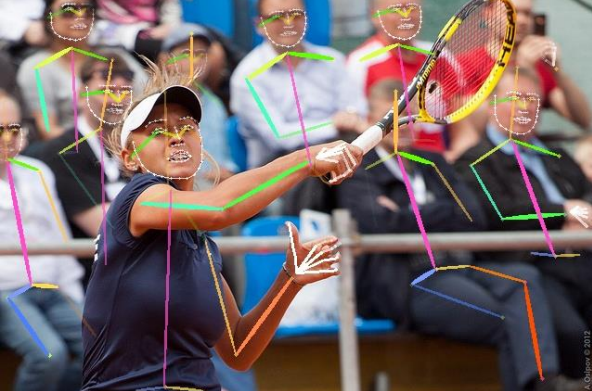
\includegraphics[width=0.75\columnwidth]{Slike/alphapic.png}
    \caption{\label{AlphaPose} Primer AlphaPose obdelane slike}
\end{figure}

    \begin{itemize}
        \item  \textbf{Simetrična integralna regresija (Symmetric Integral Keypoint Regression):} Integralna regresija je metoda prikaza izhoda konvolucijske mreže [Glej: Razlaga pojmov \ref{cnn}], ki so jo avtorji v članku \cite{regart} implementirali, kot zamenjavo za metodo "heatmap" [Glej: Razlaga pojmov \ref{heatmap}]. Ker ima metoda "heatmap" dva izstopajoča problema:

\begin{figure}[h]
    \centering
    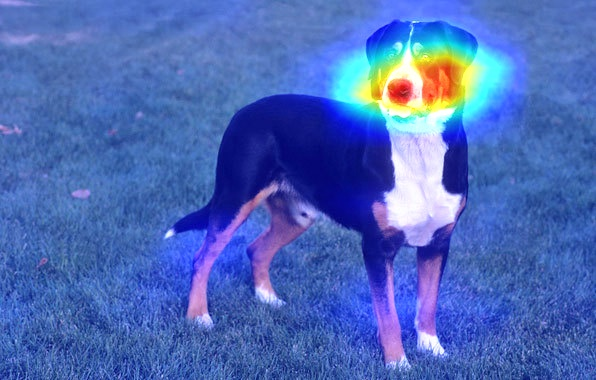
\includegraphics[width=0.75\columnwidth]{Slike/heatmap.jpg}
    \caption{\label{heatmap} Heatmap vizualizacija.}
\end{figure}

        \begin{enumerate}
            \item \textbf{Ne-odvedljivost izhoda:} "Heatmap" način predstavitve distribucije verjetnosti razredov na slikah ni zvezen in posledično ni odvedljiv. "Heatmap" je diskretna distribucija verjetnosti, saj konvolucijske nevronske mreže (CNN) podajo izhod v obliki 2-D matrike verjetnosti. \cite{regart}

            \item \textbf{Kvantizacijska napaka:} je pogojevana z načinom delovanja CNN in je neizogibna pri diskretizaciji. Kvantizacijska napaka rezultira v izgubi informacij, ki se lahko manifestira, kot slabo doloceni robovi objektov. \cite{regart}
        \end{enumerate}
        Integralna regresija je postopek razpoznavanja lokacij sklepov, ki izvira iz "heatmap" predstavitve izhoda CNN. Predstavljen je kot, z verjetnostjo vsake lokacije, utežen integral vseh lokacij na "heatmap" grafu verjetnosti. Postopek poseduje prednosti direktnega pristopa s "heatmap" grafom in pristopa z regresijo \ref{regresija}, vendar ne poseduje slabih lastnosti obeh pristopov: računska zahtevnost regresije, ne-odvedljivost "heatmap" grafa. \cite{regart}. Simetrična integralna regresija gradi na navadni integralni regresiji, s tem, da nevronska mreža upošteva prostorsko simetrijo ključnih točk (sklepov) človeškega telesa. V članku \cite{AlphaPose_clanek} je navedena, kot prva metoda na bazi regresije, ki je enako hitra in natančna, kot metode s heatmap grafom, ob tem pa izničila kvantizacijsko napako te metode.

\begin{figure}[h]
    \centering
    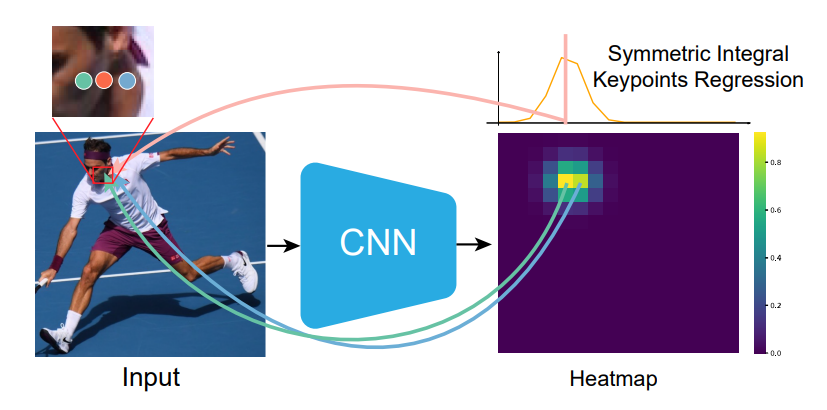
\includegraphics[width=0.75\columnwidth]{Slike/hmvssikr.png}
    \caption{\label{regresija} Vizualizacija kvantizacijske napake pristopa s heatmap-om in primerjava s simetrično integralsko regresijo.}
\end{figure}

        \item \textbf{Parametricna potlacitev nemaksimalnih vrednosti (Parametric Pose Non-Maximum-Suppression - PP-NMS):} Je algoritem za filtriranje redundantnih zaznavanj cloveskega polozaja. Narava zaznavalnikov polozaja je, da bodo poleg dejanskaga polozaja, ki ga zelimo zaznati, registrirali vec razlicic polozaja istega objekta. To se lahko zgodi zaradi delno prikritega objekta razpoznavanja ali hrupa (motenj) v sliki. Do uvedbe sistema AlphaPose so se ustvarjalci zaznavalnikov polozaja s tem problemom spopadali s povisanjem suverenosti [Glej: Razlaga pojmov \ref{suverenost}], potrebne za pozitiven izhod zaznavanja. Ta pristop rezultira v mnogih ne-zaznanih polozajih, kar je za aplikacijo zaznavanja vecjega stevila oseb nezazeljeno. Avtorji sistema AlphaPose so se problemu izbubljenih zaznavanj izognili z nizko nastavitvijo minimalne suverenosti, vendar so morali nekako popraviti problem zaznanih redundantnih polozajev. Algoritem PP-NMS za referenco izbere zaznan polozaj z najvisjim faktorjem suverenosti, polozaji, ki so po suverenosti blizu referencnemu so kandidati za eliminacijo. Odlocitev je sprejeta na bazi \textit{eliminacijskih kriterijev}, ki preverjata 2 faktorja.
            \begin{enumerate}
                \item \textbf{Podobnost:} Za dolocitev podobnosti med razlicnimi polozaji istega objekta zaznavanja oporabljamo kriterijsko funkcijo:
                \begin{equation}
                    f(P_i, P_j, \eta) = 1;[d(P_i, P_j | \Lambda, \lambda) \leq \eta]
                \end{equation}
                Kar pomeni, da je izhod enak 1, le v primeru, ko je razlika (razdalja) med polozajema $P_i$ in $P_j$ manjsa, od mejne vrednosti $\eta$. V tem primeru bo polozaj $P_i$ eliminiran zaradi redundance z referencnim polozajem $P_j$ \cite{AlphaPose_clanek}.\cite{AlphaPose_clanek}

                \item \textbf{Oddaljenost polozajev:} S to funkcijo primerjamo razdaljo med okvirji, ki dolocajo, na katerem delu slike se nahaja objekt zaznavanja polozaja. Predpostavimo, da je $B_i$ okvir polozaja $P_i$.
                \begin{equation}
                K_sim(P_i, P_j | \sigma_1) = 
                \left\{
                    \begin{array}{lr}
                        \sum_n \tanh\frac{c_i^n}{\sigma_1}, & \text{if } k_j^n\text{ is within} B(k_i^n) \\
                        
                        0, & \text{otherwise}
                    \end{array}
                \right\} 
                \end{equation}
                Kjer je $B(k_i^n)$ sredina okvirja. Operacija \verb|tanh| prefiltrira polozaje z nizkim faktorjem suverenosti. Ko imata vzajemna sklepa visok faktor suverenosti bo rezultat funkcije blizu 1, sicer pa 0 in polozaj $P_i$ bo eliminiran\cite{AlphaPose_clanek}.
            \end{enumerate}

\begin{figure}[h]
    \centering
    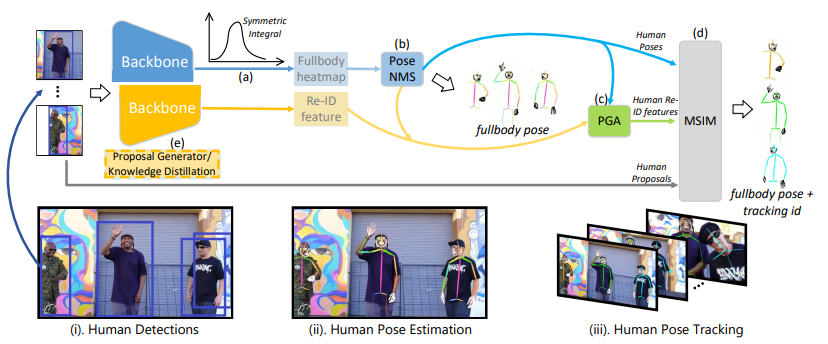
\includegraphics[width=1\columnwidth]{Slike/apfc.png}
    \caption{\label{alphapose_arhitektura} Arhitektura sistema AlphaPose.}
\end{figure}
        
    \end{itemize}

\section{Robotska roka Franka Emika Panda} je kolaborativni robot s 7 prostostnimi stopnjami [Glej: Razlaga pojmov \ref{DOF}]. Razvit je bil kot prva izmed 3 stopenj vizije podjetja, ki ga je ustvarilo (Franka Emika). Njihova vizija narekuje napredovanje kolaborativnih robotov od raziskovalnih orodij, do robotskih sodelavcev v tovarnah, do končne faze robotskega pomočnika v vsakodnevnem življenju ostarelih in obolelih ljudi. Zavoljo enostavnosti uporabe so leta 2017 predstavili sistem "Panda power tool", ki laikom omogoča učenje novih nalog v nekaj minutah in brez kakršnihkoli programerskih izkušenj. Roka ima v zadnji člen vgrajene gumbe, s pomočjo katerih lahko učimo robota z demonstracijo, torej bo robot v delovanju oponašal gibe, skozi katerega ga je uporabnik vodil z rokami. Za upravljanje z robotom na nižjem, bolj granularnem nivoju so proizvajalci robota izdali paket "Panda research package", ki omogoča dvosmerno komunikacijo med računalnikom in robotsko roko v realnem času. To uporabniku omogoča uporabo namenskih krmilnikov in po meri narejenih robotskih aplikacij. Paket vsebuje knjiznice za komunikacijo z robotom prek razlicnih programskih jezikov in \verb|franka_ROS| vmesnik za komunikacijoprek ROS [Glej: \ref{ROS}\ref{panda}] \cite{panda_website}

\begin{figure}[h]
    \centering
    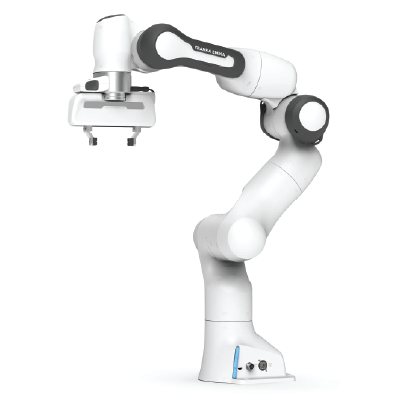
\includegraphics[width=0.75\columnwidth]{Slike/panda.png}
    \caption{\label{panda} Franka Emika Panda.}
\end{figure}

\chapter{Predelava programa AlphaPose} \label{predelava_alphapose}
Program AlphaPose ima dva nacina delovanja, deluje lahko v realnem casu, ali pa obdeluje ze posnete slike ali videoposnetke. Za svojo uporabo sem potreboval delovanje v realnem casu, vendar sem naletel na problem, saj sistem tako delovanje dovoli le z uporabo spletne kamere, ki je prek USB vodila povezano direktno na racunalnik, na katerem poganjamo program AlphaPose. Ta lastnost mi je predstavljala dva razlicna problema, in sicer:
\begin{enumerate}
    \item \textbf{Docker:} Ker je moja implementacija sistema AlphaPose morala delovati v Docker \ref{docker} okolju, je potrebno Dockerju omogociti dostop do USB vhodov in izhodov, kar nam predstavlja varnostno tveganje, saj ima Docker okolje SUDO \ref{sudo} privilegije.

    \item \textbf{ROS:} Sistem ALphaPose sem vgradil v obstojeci projekt, kjer je bil velik poudarek na samostojnosti posameznega dela resitve in enostavni integraciji v ROS \ref{ROS}. Pomembna je bila enostavna izbira kamer, kar je najenostavneje z implementacijo vsake kamere kot samostojnega vozlisca \ref{ros_node}.
\end{enumerate}
Prav tako, pa sistem AlphaPose razen lokacij posameznih cloveskih sklepov na dvodimenzionalni sliki ne podaja nobenih drugih podatkov. Za zanesljivo zaznavanje cloveskaga polozaja v robotski celici pa potrebujemo se mnogo vec podatkov, kot so globinska informacija o logaciji sklepov, lokacija kamere, koti cloveskih sklepov za kasnejse modeliranje cloveskega polozaja... V tem poglavju bom predstavil prilagoditev originalnega programa AlphaPose za odpravitev omenjenih pomanjkljivosti in za skladnost z zahtevami moje aplikacije.

\section{ROSPy integracija} Za kounikacijo za ROS \ref{ROS} je v Python program potrebno uvoziti knjiznico ROSPy. Ta knjiznica je API \ref{api}, ki nam omogoca da skozi program upravljamo s temami \ref{ros_topic}, storitvami \ref{ros_service} in parametri \ref{ros_param}. Za to knjiznico sem napisal inicializacijsko funkcijo, ki vzpostavi povezavo z vozlisci s katerimi bomo uporavljali ter definira odjemalce in ponudnike.

\begin{minted}
[
fontsize=\scriptsize
]
{python}
    def initRosPy(self):
        """
        This function initialises all of the publishers and subsribers
        required by the program.

        Args
        ----
            color_topic(str) : ROS topic publishing color images, used by AlphaPose

            depth_topic(str) : ROS topic publishing depth images, used to determine 3D location of joints
        """
        rospy.init_node("vision", anonymous = True)

        rospy.Service(self.poseNode, SetBool, self.enablePoseCB)
        rospy.Service(self.camPoseNode, SetBool, self.enableCamPoseCB)
        rospy.Service(self.camSelectPanda, SetBool, self.selectPandaCB)

        self.create_service_client(self.poseNode)
        self.create_service_client(self.camPoseNode)
        self.create_service_client(self.camSelectPanda)

        self.pub_TRANS_POSE = tf2_ros.TransformBroadcaster()
        self.transmsg = geometry_msgs.msg.TransformStamped()
        self.tfbuffer = tf2_ros.Buffer()
        self.tflistener = tf2_ros.TransformListener(self.tfbuffer)
        self.camInfo('/realsense_top/color')
        
        self.maxDEPTH = rospy.get_param("/realsense_top/aligned_depth_to_color/image_raw/compressedDepth/depth_max") # Za kasnejse mapiranje globine
        while True:
            if self.colorTopic != None:
                break
        
        self.sub_POSE = rospy.Subscriber(self.colorTopic, Image, self.pose_CB)
        self.sub_DEPTH = rospy.Subscriber(self.depthTopic, Image, self.depth_CB)

        self.pub_POSE = rospy.Publisher("/alphapose_pose", Image, queue_size=1)
        self.pub_DEPTH = rospy.Publisher("/alphapose_depth", Image, queue_size=1)
        self.pub_MARKER = rospy.Publisher("/reconcell/markers", MarkerArray, queue_size=1)
\end{minted}
\newpage
 V njej definiramo storitve za omogocenje/onemogocenje programa AlphaPose, kalibracijske funkcije za polozaj kamere in izbiro kamere. Te storitve omoocajo programu, da spreminjamo njegove parametre, ne da bi ga ponovno zagnali, kar omogoci, da YOLOv3 nevronska mreza, ki jo program AlphaPose uporablja za dolocanje cloveskega polozaja, ostane nalozena v spominu graficne kartice. Dovoljuje nam tudi zacasno pavziranje pretoka informacij, kar sprosti pasovno sirino vodila ROS za bolj casovno kriticne aplikacije.

 Prva pomanjkljivost AlphaPose, ki sem jo moral odpraviti je bila prejemanje slik z ROS vozlisca kamere, odpravil sem jo tako, da sem zaobsel DataLoader in jo z orodjem \verb|CvBridge().imgmsg_to_cv2| pretvoril iz formata ROS slikovnega sporocila (\verb|sensor_msgs.Image|)\ref{ROS_img}, ki je v obliki seznama 8-bitnih kodiranih vrednosti, zato ima objekt ROS slikovnega sporocila vkljuceno se spremenljivko \verb|step|, ki vsebuje dolzino vrstice, kar pomaga pri kasnejsi razclenitvi seznama.Pretvoril sem jo v format knjiznice \verb|OpenCV|, ki je n-dimenzionalna matrika, povzeta poobjektu \verb|np.ndarray| iz knjiznice \verb|Numpy|. Ta format za opisovanje slik uporablja knjiznica pytorch, v kateri je zgrajen sistem AlphaPose.

\begin{figure}[h]
    \centering
    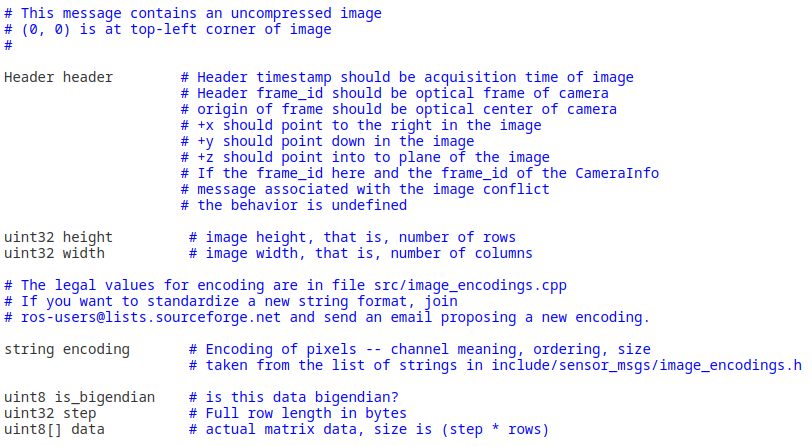
\includegraphics[width=0.75\columnwidth]{Slike/sensor_msg_image.png}
    \caption{\label{ROS_img} Format ROS slikovnega sporocila.}
\end{figure}

\begin{figure}[h]
    \centering
    
\includegraphics[width=0.7\columnwidth]{Slike/matrix_Mat_object.png}
    \caption{\label{ROS_img} Format OpenCV slike (np.ndarray, vendar v programu uporabljamo le dvodimenzionalne)}
\end{figure}


 ROSPy za prejemanje datotek z ROS tem \ref{ros_topic} uporablja tako imenovane povratne (\textit{callback}) funkcije. Te funkcije se uporabljajo za izvedbo dolocene operacije ob nekem dolocenem dogodku, v nasem primeru je to pojav nove slike na slikovni temi, ki jo spremljamo, oz. "poslusamo". Uporaba teh funkcij omogoca asinhrono delovanje programa, vendar AlphaPose ni misljen za tak nacin delovanja, zato sem moral njegovo delovanje razdeliti na inicializacijski del, ki ob prvotnem zagonu programa nalozi nevronsko mrezo in njene utezi ter na obdelovalni del, kjer poteka dejanska zaznava cloveskega polozaja na prejeti sliki.

 Na projektu, na katerem sem delal je implementacija strojnega vida bila izvedena s stereoskopsko kamero intel Realsense, za katero obstaja ROS ovoj \ref{ROS_wrapper}. Ta integracijska plast objavlja barvno in globinsko sliko na razlicni temi, torej sem za njuno prebiranje potreboval dve loceni povratni funkciji, barvno sliko sem posredoval funkciji za zaznavanje cloveskega polozaja, ki je bila prilozena z API sistema AlphaPose, iz globinske slike pa sem nato prebiral podatke s katerimi sem izracunaval oddaljenosti od robotov in polozaje sklepov.

 \begin{itemize}
     \item \textbf{Barvna slika:} Za pridobivanje barvne slike je zadolzena povratna funkcija \verb|pose_CB|. Ta funkcija sprejeto sliko najprej pretvori iz ROS slikovnega sporocila v format \verb|openCV|, nato jo posreduje sistemu AlphaPose, ki nam vrne Pyhon slovar, ki vsebuje lokacije sklepov na sliki v obliki (x, y) \textbf{TOODO: format alphapose outputa}. Nato se 'sprehodi' skozi prejeti slovar s parom \verb|for| zank in njihove x in y vrednosti zapise v drug slovar, ki je bil zasnovan specificno za namene preslikave cloveka v robotsko vizualizjsko orodje RViz, ki je del sistema ROS.

\begin{listing}[H]
\begin{minted}
    [
    fontsize=\scriptsize
    ]
    {python}
        self.body ={'R_ankle': {'x': None, 'y': None, 'z': None, 'pf': 'r_knee_default', 
            'cf': 'r_ankle_default','rot_x': False, 'rot_y': False, 'rot_z': False, 'lower_j': None, 
            'parent': 'R_knee','transj': [0, 0, -0.44], 'qx': np.ndarray(5), 'qy': np.ndarray(5), 'qz': np.ndarray(5), 
            'worldx': None, 'worldy': None, 'worldz': None},
\end{minted}
\caption{Primer opisa sklepa v namenskem slovarju}
\end{listing}
\newpage
\begin{listing}[H]
\begin{minted}
[
fontsize=\scriptsize
]
{python}
def pose_CB(self, input):
    if self.enablePose and self.camSel:
        self.img_POSE = CvBridge().imgmsg_to_cv2(input, desired_encoding='rgb8')
        
        self.IMAGE_HEIGHT = self.img_POSE.shape[0]
        self.IMAGE_WIDTH = self.img_POSE.shape[1]
        self.pose = self.process("demo", self.img_POSE)
        self.vis_POSE = self.vis(self.img_POSE, self.pose)
    
        if self.pose != None:
            self.keypoints = self.pose['result'][0]['keypoints']
    
            self.secs = str(input.header.stamp)[:10]
            self.nsecs = str(input.header.stamp)[10:]
    
            jIgnore = ['waist', 'torso', 'body']
            tagIgnore = ['roll', 'pitch', 'yaw']
            for key, joint in self.body.items():
                keySegs = key.split('_')
                if keySegs[0] not in jIgnore:
                    if keySegs[-1] not in tagIgnore:
                        joint['x'] = int(self.keypoints[16-i][0])
                        joint['y'] = int(self.keypoints[16-i][1])
            self.assignVirtualJoints()   
            
            if self.args.circles == True:
                self.vis_POSE = cv2.circle(self.vis_POSE, (self.body['L_wrist']['x'], self.body['L_wrist']['y']), radius=10, color=(255, 0, 255), thickness=2)
                self.vis_POSE = cv2.circle(self.vis_POSE, (self.body['R_wrist']['x'], self.body['R_wrist']['y']), radius=10, color=(255, 0, 255), thickness=2)
            
        else:
            print(f"{Fore.RED} No pose detected...")
            
        if self.enableCamPose == True and self.colorTopic == '/realsense_top/color/image_raw':
            self.vis_POSE = self.markerHandler(image=self.vis_POSE)
        self.markerPub()
        
        self.out_POSE = CvBridge().cv2_to_imgmsg(self.vis_POSE, encoding = 'rgb8')
        self.pub_POSE.publish(self.out_POSE)

\end{minted}
\caption{pose\_CB povratna funkcija}
\end{listing}

    \item \textbf{Globinska slika:} Za pridobitev globinska slike je zadolzena povratna funkcija \verb|depth_CB|, ki prav tako kot prejsnja povratna funkcija najprej pretvori sliko iz formata slikovnega sporocila v \verb|openCV| format. V globinskih slikah s kamere realsense so globine posameznih pisklov predstavljene s sivinskimi nivoji, kjer je sivinski nivo piksla enak njegovi globini v milimetrih. Piksel oddaljen 5m bi torej imel sivinski nivo 5000, na 
    16-bitni lestvici kjer je 0 popolnoma crno, 65536 pa popolnoma belo. Vendar stereoskopske globinske kamere ustvarjajo artefakte v obrisih, kar se prikaze kot popolnoma crna obroba predmetov na sliki. Za minimizacijo vpliva teh artefaktov sem globinsko sliko pred uporabo zameglil. Glavna naloga te povratne funkcije je razbiranje globinskih vrednosti posameznih sklepov, funkcija kot vhod prejme slovar s polozaji posameznih sklepov, nato se skozi ta slovar sprehodi s pomocjo \verb|for| zanke in za vsak par (x,y) koordinat prebere sivinsko vrednost piksla s tema koordinatama in jo doda v slovar. 


\begin{listing}[!ht]
\begin{minted}
[
fontsize=\scriptsize
]
{python}
def depth_CB(self, input):    
    if self.enablePose and self.camSel:
        self.img_DEPTH = CvBridge().imgmsg_to_cv2(input, desired_encoding='16UC1')
        if self.img_DEPTH.shape[0] != self.IMAGE_HEIGHT:
            self.img_blur_DEPTH = cv2.resize(self.img_DEPTH, dsize=[self.IMAGE_WIDTH, self.IMAGE_HEIGHT])
            self.highRes = True
        else:
            self.img_blur_DEPTH = cv2.GaussianBlur(self.img_DEPTH, (5,5), cv2.BORDER_DEFAULT)
            self.highRes = False

        if self.camPose != None and self.camSel == True:
            self.SendTransform2tf(p=self.camPose,q=self.camRot, parent_frame="/world", child_frame=self.tfFrame)
                    
        if self.pose != None:
            for key, joint in self.body.items():
                if joint['y'] >= self.IMAGE_HEIGHT:
                    joint['z'] = self.img_blur_DEPTH[self.IMAGE_HEIGHT-1, int(joint['x'])]/1000
                elif joint['x'] >= self.IMAGE_WIDTH:
                    joint['z'] = self.img_blur_DEPTH[int(joint['y']), self.IMAGE_WIDTH-1]/1000
                else:
                    joint['z'] = self.img_blur_DEPTH[int(joint['y']), int(joint['x'])]/1000
               
                joint['qx'] = np.roll(joint['qx'], -1)
                np.put(joint['qx'], 4, joint['x'])
                        
                joint['qy'] = np.roll(joint['qy'], -1)
                np.put(joint['qy'], 4, joint['y'])
                        
                joint['qz'] = np.roll(joint['qz'], -1)
                np.put(joint['qz'], 4, joint['z'])

            print(f"{Fore.CYAN}LEFT:\nDEPTH: {self.body['L_wrist']['z']} | LOCATION: {self.body['L_wrist']['x'], self.body['L_wrist']['y']}")
            print(f"{Fore.MAGENTA}RIGHT:\nDEPTH: {self.body['R_wrist']['z']} | LOCATION: {self.body['R_wrist']['x'], self.body['R_wrist']['y']}")

            self.maxdepth_loc, self.mindepth_loc = np.unravel_index(np.argmax(self.img_blur_DEPTH),self.img_blur_DEPTH.shape), np.unravel_index(np.argmin(self.img_blur_DEPTH), self.img_blur_DEPTH.shape)


            self.rounddepth_L = str(self.body['L_wrist']['z'])[:4]
            self.rounddepth_R = str(self.body['L_wrist']['z'])[:4]

            print(f"{Fore.GREEN} Max depth: {self.maxdepth_loc} {Fore.RED} | Min depth: {self.mindepth_loc}")
            
\end{minted}
\end{listing}

\begin{listing}[H]
\begin{minted}
[
fontsize=\scriptsize
]
{python}
    for key, joint in self.body.items():
                jointx = self.GetMoveAvg(joint['qx'])        
                jointy = self.GetMoveAvg(joint['qy'])
                jointz = self.GetMoveAvg(joint['qz'])
               
                jointxyz = self.uv_to_XY(jointx, jointy, jointz)

                

                if joint['cf'] != None:
                    self.SendTransform2tf(p=jointxyz, parent_frame=self.tfFrame, child_frame=(joint['cf']+'/rs'))
                    if key == 'body':
                        transToWorld = self.GetTrans('world',joint['cf']+'/rs')

                        self.SendTransform2tf(p=transJoint, parent_frame=joint['pf'], child_frame=joint['cf'])
                    else: 
                        transToWorld = self.GetTrans('world',joint['cf']+'/rs')
                
                        worldPos = transToWorld.translation
                        
                        joint['worldx'] = -worldPos.x
                        joint['worldy'] = -worldPos.y
                        joint['worldz'] = -worldPos.z

                        jointRot = self.getRot(joint=key)
                        if joint['transj'] != None:
                            transJoint = joint['transj']
                        else:
                            transJoint = [0,0,0]
                        self.SendTransform2tf(p=transJoint, q=jointRot, parent_frame=joint['pf'], child_frame=joint['cf'])
                        
            if self.args.circles == True:
                
                self.circle_DEPTH = cv2.circle(self.img_blur_DEPTH, (self.body['L_wrist']['x'], self.body['L_wrist']['y']), radius=10, color=(255, 0, 255), thickness=2)
                self.circle_DEPTH = cv2.circle(self.circle_DEPTH, (self.body['R_wrist']['x'], self.body['R_wrist']['y']), radius=10, color=(255, 0, 255), thickness=2)
                self.out_DEPTH = CvBridge().cv2_to_imgmsg(self.circle_DEPTH, encoding = '16UC1')

        else:
            self.out_DEPTH = CvBridge().cv2_to_imgmsg(self.img_DEPTH, encoding = '16UC1')

        self.pub_DEPTH.publish(self.out_DEPTH)
        if self.colorTopic == '/realsense_top/color/image_raw':
            self.visMarker()
        self.getProximity()
\end{minted}
\caption{depth\_CB povratna funkcija}
\end{listing}
\end{itemize}
\newpage


\section{Dolocitev cloveskega polozaja} Velik del ideje za uporabo strojnega vida pri zagotavljanju varnosti v kolaborativni robotiki je bila hitra in neobcutljiva postavitev sistema. Pri uporabi npr. svetlobne zavese za zagotavljanje varnosti moramo biti pazljivi pri orientaciji modulov svetlobnih zaves, kjer moramo paziti na poravnanost in zagotavljanje jasnega vidnega polja med polovicama svetlobne zavese. Med drugim mrajo biti moduli postavljeni na specificni razdalji, ki jo je tezko spreminjati ob spremembi potreb robotske celice, kar je cedalje bolj perec problem v industriji, ki stremi k vedno bolj dinamicnemu in modularnemu pristopu do robotskega dela. Ta sprememba smernic je se posebej razvidna na hitro rastocem podrocju sodelujocih robotov. Za razliko od fiksnih sistemov s svetlobnimi zavesami ali detektorji cloveske prisotnosti, lahko z uporabo strojnega vida dolocamo clovesko oddaljenost od delovnega prostora robota iz prakticno katerekoli tocke, kjer sta razvidna tako clovek, kot celica. Tako lahko kamero za zaznavo postavimo ktakorekoc kamorkoli, kjer je ta pogoj izpolnjen, vendar pa to s seboj prinese tudi slabosti. Ko uporabniku omogocimo prosto premikanje kamere izgubimo pozicijsko tocnost fiksno postavljene kamere, kar je bistven podatek za kakrsnokoli merjenje razdalje na slikah.

\subsection{Dolocitev polozaja kamere} Za kakrsnokoli zanesljivost podatkov o razdalji med clovekom in roboti je nujno potreben natancen podatek o polozaju kamere. Na mojem projektu sta bili na voljo 2 kameri, od katerih je ena bila namescena na koncu robotske roke, torej je dolocitev njenega polozaja bila trivialna, saj je bila dolocena s transformacijsko matriko od zadnjega clena robotske roke. Druga kamera je bila namescena pod stropom na lokaciji, ki bi jo bilo izjemno tezko dolociti z rocnimi meritvemi, zato sem se za dolocanje polozaja kamere odlocil uporabiti ArUco markerje. ArUco markerji so podvrsta takoimenovanih "fiducial" oziroma referencnih markerjev, to so racunalniku enostavno razpoznavni vzorci s tocno dolocenimi dimenzijami, na podlagi katerih lahko dolocimo velikost, oddaljenost in orientacijo predmeta na sliki. 

\begin{figure}[H]
    \centering
    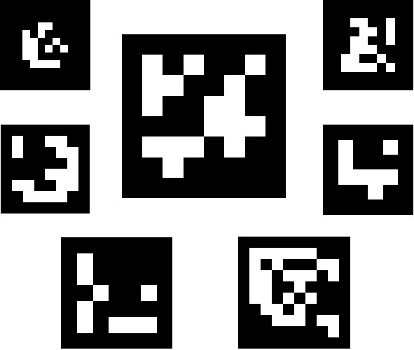
\includegraphics[width=0.5\columnwidth]{Slike/markers.jpg}
    \caption{\label{ArUco_markers} Primer ArUco markerjev}
\end{figure}

Na robotsko delovno povrsino sem na lokacije, ki so bile stratesko izbrane za vidljivost med robotskim delovanjem s pomocjo 3D natisnjne sablone nalepil nabor ArUco markerjev, v program sem vnesel njihove polozaje glede na bazni koordinatini sistem robotske celice, nato pa jih zaznal z uporabo knjiznice openCV ArUco, ki je vrnila polozaje njihovih kotov glede na koordinatni sistem kamere (2D informacija). Iz znanih razdalj med markerji v realnem svetu in njihovih projekcij na senzor kamere sem nato z uporabo algoritma n-tockovne perspektive dolocil polozaj kamere glede na bazni koordinatni sistem kamere.

\begin{align} \begin{bmatrix} u \\ v \\ 1 \end{bmatrix} &= \bf{A} \hspace{0.1em} \Pi \hspace{0.2em} ^{c}\bf{T}_w \begin{bmatrix} X_{w} \\ Y_{w} \\ Z_{w} \\ 1 \end{bmatrix} \\ \begin{bmatrix} u \\ v \\ 1 \end{bmatrix} &= \begin{bmatrix} f_x & 0 & c_x \\ 0 & f_y & c_y \\ 0 & 0 & 1 \end{bmatrix} \begin{bmatrix} 1 & 0 & 0 & 0 \\ 0 & 1 & 0 & 0 \\ 0 & 0 & 1 & 0 \end{bmatrix} \begin{bmatrix} r_{11} & r_{12} & r_{13} & t_x \\ r_{21} & r_{22} & r_{23} & t_y \\ r_{31} & r_{32} & r_{33} & t_z \\ 0 & 0 & 0 & 1 \end{bmatrix} \begin{bmatrix}\label{PNP} X_{w} \\ Y_{w} \\ Z_{w} \\ 1 \end{bmatrix} \end{align}

Zgornja funkcija je transformacija tocke iz koordinatnega sistema sveta v koordinatni sistem kamere, kjer so \begin{math} X_W, Y_W \end{math} in \begin{math} Z_W\end{math} koordinate tocke v baznem koordinatnem sistemu, \begin{math} f_x \end{math} in \begin{math} f_y \end{math} goriscni razdalji kamere, \begin{math} c_x \end{math} in \begin{math} c_y \end{math} pa opticna centra koordinatnega sistema kamere. \begin{math} U \end{math} in \begin{math} V \end{math} predstavljata lokacijo projekcije tocke na ravnino senzorja kamere, \begin{math} r_11 \end{math} do \begin{math} r_33 \end{math} predstavljajo rotacijsko matriko transformacije, \begin{math} t_x. t_y \end{math} in \begin{math} t_z \end{math} pa so komponente translacijskega vektorja od tocke v koordinatnem sistemu sveta do koordinatnega sstema kamere.

Za dolocitev polozaja kamere je potreben inverz zgornje funkcije, vendar nam le-ta lahko vrne dvoumno resitev, ce vanjo vnesemo le minimalno stevilo tock (3). Ta pojav je znan kot dvoumnost 3-tockovne perspektive, za resitev tega fenomena pa sem uporabil 6 markerjev, kar je rezultiralo v sorazmerno natancni enolicni resitvi. Vendar pa je zaradi locljivosti kamere in relativno velike oddaljenosti rezultat bil nekoliko zamaknjen, zato sem napisal funkcijo, ki je poskrbela, da se zaznani polozaji markerjev ujemajo z znanimi.

\begin{listing}[H]
\begin{minted}
[
fontsize=\scriptsize
]
{python}
def CamPoseCorrection(self, initial_pose:list)->list:
        errorx = []
        errory = []
        errorz = []
        for key, coords in self.cornerDict.items():
            if coords != None:
                topRc = coords[0]
                botLc = coords[2]
                cx = (botLc[0]+topRc[0])/2
                cy = (botLc[1]+topRc[1])/2
                cz = self.img_blur_DEPTH[int(cy), int(cx)]/1000
                visMarkerloc = self.uv_to_XY(cx, cy, cz)
                self.SendTransform2tf(p=visMarkerloc, parent_frame='rs_top', child_frame=('markerVis/'+str(key)))

                # Calculate center of corresponding marker in real world coordinates
                topRw = self.markerDict[key][0]
                botLw = self.markerDict[key][2]
                wx = (botLw[0]+topRw[0])/2
                wy = (botLw[1]+topRw[1])/2
                wz = botLw[2]

                # Get real world coordinates from cameras view of the markers
                worldloc = self.tfbuffer.lookup_transform('world','markerVis/'+str(key), time=rospy.Time())
                wcx, wcy, wcz = worldloc.transform.translation.x, worldloc.transform.translation.y, worldloc.transform.translation.z

                errorx.append(wx-wcx)
                errory.append(wy-wcy)
                errorz.append(wz-wcz)
        # Get mean error for each axis
        mx = np.mean(errorx)
        my = np.mean(errory)
        mz = np.mean(errorz)
        
        return [initial_pose[0]+mx, initial_pose[1]+my, initial_pose[2]+mz]
\end{minted}
\caption{Funkcija za samodejno korekcijo polozaja kamere}
\end{listing}





\chapter{Razlaga pojmov} \label{razlaga_pojmov}
\begin{itemize}
    \item \textbf{Heatmap:} \label{heatmap} je nacin vizualizacije podrocja na sliki, ki ga konvolucijska nevronska mreza (CNN) povezuje s specificnim izhodnim razredom. Znan je tudi pod okrajšavo CAM (Class Activation Mapping), uporablja se za, človeku - prijazno, vizualizacijo distribucije verjetnosti, da je na sliki objekt dolocenega razreda razpoznavanja. \cite{heatmap_website}

    \item \textbf{Konvolucijske nevronske mreze:} \label{cnn}so vrsta nevronske mreže, namenjene pretežno za obdelavo slik. Glavni cilj konvolucijskih nevronskih mrež je naučiti se lokalne in globalne značilnosti vhodnih slik, kar omogoča, da lahko mreža klasificira, zaznava in segmentira objekte v slikah. Konvolucijske nevronske mreže uporabljajo konvolucijske plasti za izvajanje filtriranja vhodnih podatkov z matričnimi filtri (kernel). Filtri se običajno uporabljajo za zaznavanje robov, tekstur in drugih vizualnih značilnosti, ki so pomembne za prepoznavanje objektov na sliki. \cite{cnn_clanek}

    \item \textbf{Suverenost (confidence):} \label{suverenost} V polju zaznavanja cloveskega polozaja je suverenost metrika, ki nam pove verjetnost pravilnosti zaznanega polozaja in je dobra kriterijska metrika za detektorje polozaja. Tipicno jo predstavimo, kot skalarno vrednost med 0 in 1, kjer 1 pomeni 100\% prepricanost v pravilnost zaznanega polozaja, 0 pa popolno prepricanost, da je polozaj napacno zaznan. Suverenost je izracunana na bazi vecih faktorjev, kot so: kvaliteta vhodne slike, kompleksnost oblike in teksture objekta zaznavanja in točnost algoritma. \cite{confidence_clanek}\cite{confidence_website}

    \item \textbf{Regresija:} \label{regresija }\textbf{TODO}

    \item \textbf[Docker:] \label{docker} \textbf{TODO}

    \item \textbf[SUDO:] \label{sudo} \textbf{TODO}

    \item \textbf[API:] \label{api} \textbf{TODO}

    \item \textbf[ROS ovoj:] \label{ROS_wrapper} \textbf{TODO}



    \item \textbf{Prostostna stopnja:} \label{DOF}V robotiki nam stevilo prostostnih stopenj pove s kolikimi neodvisnimi spremenljivkami lahko opisemo polozaj vrha robota. Opisujejo lahko translatorno ali rotacijsko gibanje. V vecini primerov je stevilo prostostnih stopenj robotskega manipiulatorja enako stevilu njegovih sklepov. \cite{DOF_website}

    \item \textbf{Realni cas (Real-time):}\label{RealTime} Obdelava v realnem casu je pojem, rezerviran za sisteme, ki zagotavljajo odziv znotraj specificiranega casovnega intervala. Ko govorimo o delovanju v realnem casu so ti intervali reda milisekund ali vcasih mikrosekund. Sisteme, ki delujejo v realnem casu, glede na posledice zamujenega casovnega intervala lahko locimo na 3 skupine:
    \begin{itemize}
        \item \textbf{Trdi sistemi:} Zamujen casovni interval rezultira v popolnem sistemskem zastoju.
        \item \textbf{Cvrsti sistemi:} Lahko tolerirajo obcasno zamujen casovni interval,vendar to lahko rezultira v poslabsanju kvalitete opravljanja zadane naloge, saj je rezultat po zamujenem casovnem intervalu neuporaben.
        \item \textbf{Mehki sistemi:} Po zamujenem casovnem intervalu upade uporabnost rezultata in s tem upade tudi kakovost delovanja sistema.
    \end{itemize}

\begin{figure}[h]
    \centering
    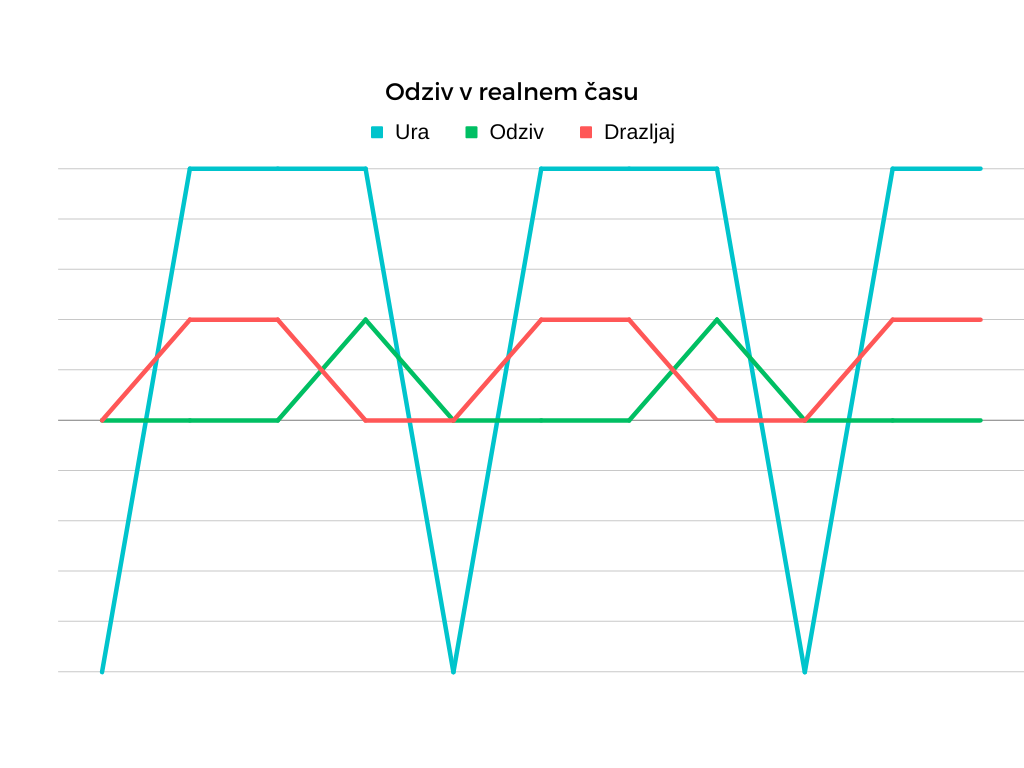
\includegraphics[width=0.75\columnwidth]{Slike/Untitled design (1).png}
    \caption{\label{RealTime} Prikaz odziva sistema v fiksnem časovnem intervalu.}
\end{figure}



    
\end{itemize}


\cleardoublepage\phantomsection\addcontentsline{toc}{chapter}{Literatura} % vnos literature v kazalo

% 1. način: BibTeX
\bibliographystyle{ieeetrslo}
\bibliography{literatura}

\end{document}